\section{Task 2: Frequency}
\subsection{Approach}
\begin{frame}{Task 2: Frequency}
	\framesubtitle{Ansatz}
	\begin{center}
		Small Oscillations around Steady-State
		\begin{equation*}
			\theta_e = 0 \quad \theta_e = \arccos\left(\frac{1}{\omega^2}\frac{g}{L}\frac{(m_1+m_2)}{m_2}\right)
		\end{equation*}
		Approximation with spring-mass-equation
		\begin{equation*}
			m\ddot{x} = -kx
		\end{equation*}
	\end{center}
\end{frame}


\subsection{Result}
\begin{frame}{Task 2: Frequency}
	\framesubtitle{Result}
	\begin{center}
		\begin{equation*}
			\Delta \ddot{\theta} = \frac{m_2\cos(2\theta_e)\omega^2 - \frac{g}{L}\cos(\theta_e)(m_1+m_2)}{m_1(1-\cos(2\theta_e))+m_2}\Delta \theta
		\end{equation*}
		\begin{align*}
			\omega_e =
			\sqrt{\frac{m_2\omega^2(g^2(m_1 + m_2)^2-L^2m_2^2\omega^4)}{2g^2m_1(m_1+m_2)^2-L^2m_2^2\omega^4(2m_1+m_2)}} 
		\end{align*}
		Edge Case: $m_1 = 0$
		\begin{equation*}
			\omega_e = \sqrt{\frac{L^2\omega^4 - g^2}{L^2\omega^2}}
		\end{equation*}
	\end{center}
\end{frame}

\subsection{Verification with simulation}
\begin{frame}{Task 2: Frequency}
	\framesubtitle{Verification with simulation}
	\begin{figure}[H]
		\centering
		$m_1 = 1\,\left[\mathrm{kg}\right]$, $m_2 = 2\,\left[\mathrm{kg}\right]$, $L = 0.4\,\left[\mathrm{m}\right]$, $\omega = 3\pi\,\left[\mathrm{\frac{rad}{s}}\right]$, $x_0 = \left(\begin{array}{c c}
		1 & 0
		\end{array}\right)^T \quad \text{Matlab: }1.01\,\left[\mathrm{Hz}\right]$\\ [0.5cm]
		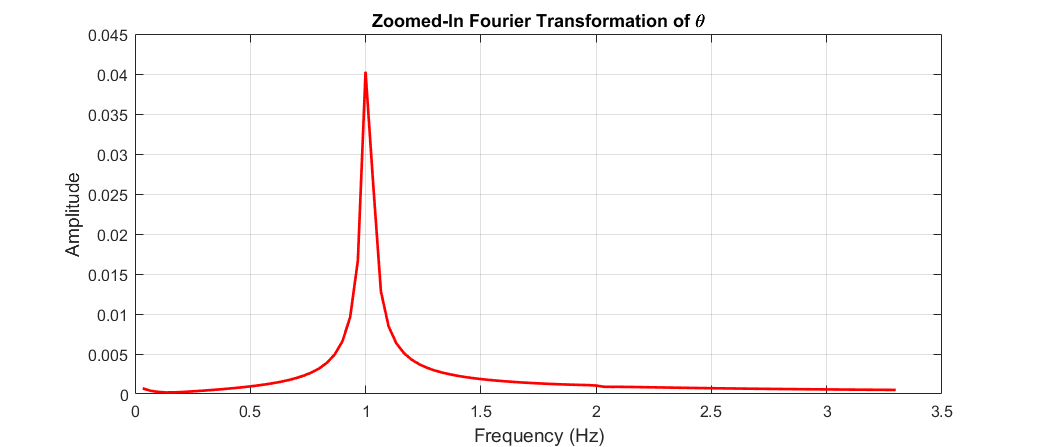
\includegraphics[width=1\textwidth]{pics/frequency.png}
	\end{figure}
\end{frame}